\subsection*{Disclaimer}
In this report, I adopt a writing convention:
\begin{itemize}
    \item Filenames are in \textit{italic}
    \item Any value, variable, string, object ... is in \textbf{boldface} 
\end{itemize}
Please note that the output files are quite big, I will provide the first ten results of each language in the report, the complete list of results will be available on the \href{https://github.com/PaxOwl/big-data-project}{github page} of this project in \textit{project/data\_out/}.
\section{Introduction}
In the late 90's, several search engine were in competition about speed and efficiency. In 1998, Larry Page and Sergey Brin put an end to the race with the PageRank algorithm and their search engine: Google. This algorithm makes use of the hyperlinks between the pages. It assigns a score to a page depending on the number of times a user could go to the page by clicking on random links. It is a measure of the centrality of the web.

In this work we will look into 2 approach for this algorithm: the matrix approach which is the resolution of an eigenproblem, and an approach using the power iteration methods.

This algorithm will be tested to rank all the pages of Wikipedia in 2013 (separated by language) in 24 different languages. It could then lead to a study about the rank of a page in different languages.

The CPU will be monitored at all time during the computation to keep a precise track of what task is fast/slow and where to improve the code.
\newpage
\section{Task 1}
\label{sec:task1}
In Graph Theory, a graph is a structure made of vertices connected by edges. These graph can be directed (asymmetrically) and undirected (symmetrically). The PageRank method uses the graph theory to rank pages of the web by analyzing the hyperlinks between pages. In this part we will see how this algorithm works from a matrix approach using the following graph.

\begin{figure}[htbp]
    \centering
    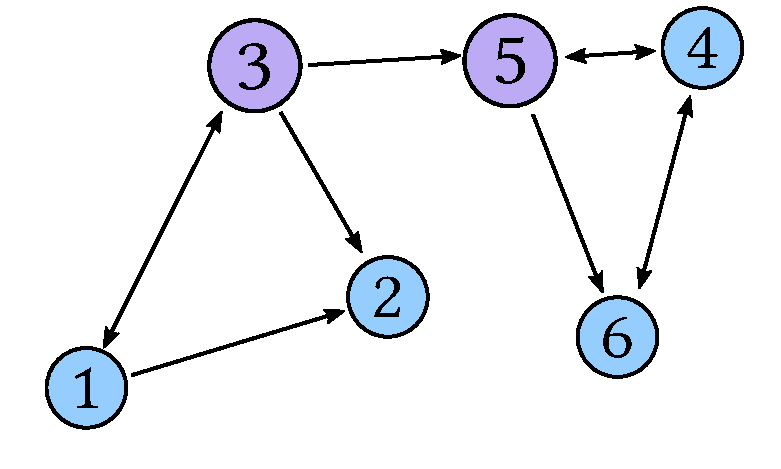
\includegraphics[width=.5\linewidth]{network.pdf}
    \caption{Graph used to experiment with the algorithm}\label{fig:network}
\end{figure}

The first mathematical object needed is the adjacency matrix. It is a matrix encoding the structure of the graph. This matrix is defined by:
\begin{equation}
    A_{ij} = \left\{\begin{array}{ll}
        1 & $if $j$ point to $i\\
        0 & \text{otherwise}
    \end{array} \right.
\end{equation}
The adjacency matrix of the considered graph is:
\[
    \begin{pmatrix}
        0 & 0 & 1 & 0 & 0 & 0\\
        1 & 0 & 1 & 0 & 0 & 0\\
        1 & 0 & 0 & 0 & 0 & 0\\
        0 & 0 & 0 & 0 & 1 & 1\\
        0 & 0 & 1 & 1 & 0 & 0\\
        0 & 0 & 0 & 1 & 1 & 0\\
    \end{pmatrix}
\]
Since our graph is directed, this matrix is not symmetrical.

Once the adjacency matrix is build, we need the stochastic matrix:
\begin{equation}
    S_{ij} = \left\{ \begin{array}{ll}
        A_{ij} / k_j^{\text{out}} & \text{if } k_j^{\text{out}} \neq 0\\
        1 / N & \text{otherwise} 
    \end{array} \right. \text{ with } k_j^{\text{out}} = \displaystyle\sum_{i=1}^{N} A_{ij}
\end{equation}
The out-degree $k_j^{\text{out}}$ corresponds to the number of vertices to leave the vertex $j$. An element $S_{ij}$ of the stochastic matrix corresponds to the probability of jumping from node $i$ to node $j$. The second part in the definition of $S$ in case we end up on a node without any way out ($k_{\text{out}} = 0$). In that case we have a probability $1/N$ of jumping into any node of the network.

The out-degree $k^{\text{out}}$ and the stochastic matrix $S$ of the considered graph are:
\[  
    k^{\text{out}} = \begin{pmatrix}
        2\\
        0\\
        3\\
        2\\
        2\\
        1\\
    \end{pmatrix}
    \qquad \qquad
    S = \begin{pmatrix}
        0 & 1/6 & 1/3 & 0 & 0 & 0\\
        1/2 & 1/6 & 1/3 & 0 & 0 & 0\\
        1/2 & 1/6 & 0 & 0 & 0 & 0\\
        0 & 1/6 & 0 & 0 & 1/2 & 1\\
        0 & 1/6 & 1/3 & 1/2 & 0 & 0\\
        1 & 1/6 & 0 & 1/2 & 1/2 & 0\\
    \end{pmatrix}
\]
Now that we have the probability to jump into a node $j$ from any node $i$, we can define the initial probability distribution $\mathbf{p}^{(0)}$ which depends on the starting node $j_0$.
\begin{equation}
    p_i^{(0)} = \delta_{ij_0}
\end{equation}

Let us introduce the Perron-Frobenius operator $G$:
\begin{equation}
    G_{ij} = \alpha S_{ij} + (1 - \alpha) v_i
\end{equation}
Where $\alpha$ is the damping factor and \textbf{v} a preferential vector. By convention, we take $\alpha = \num{0.85}$, but it could be anything in the interval $[0.5, 1[$. The values of the preferential vector \textbf{v} are all the same: $v_i = 1/N$.

By applying $G$ onto \textbf{p} an infinite number of time (i.e. $G^{\infty}\mathbf{p}^{(0)}$) we find the steady state probability distribution \textbf{P}.

The computation of the Google matrix in the example network gives:
\begin{equation}
    G = \begin{pmatrix}
        0.025 & 1/6 & 0.308 & 0.025 & 0.025 & 0.025\\
        0.450 & 1/6 & 0.308 & 0.025 & 0.025 & 0.025\\
        0.450 & 1/6 & 0.025 & 0.025 & 0.025 & 0.025\\
        0.025 & 1/6 & 0.025 & 0.025 & 0.450 & 0.875\\
        0.025 & 1/6 & 0.208 & 0.450 & 0.025 & 0.025\\
        0.025 & 1/6 & 0.025 & 0.451 & 0.451 & 0.025\\
    \end{pmatrix}
\end{equation}

Once we have \textbf{P}, we have to sort it in decreasing order and we have the ranking of our network. We now have all that is needed to solve the eigenproblem and rank the network.


After solving the eigenproblem, the results are as follows:

\begin{table}[htbp]
    \begin{minipage}{.25\linewidth}
        \centering
        \begin{tabular}{ll}
            \toprule
            Node & Rank\\
            \midrule
            4 & 1\\
            6 & 2\\
            5 & 3\\
            2 & 4\\
            3 & 5\\
            1 & 6\\
            \bottomrule
        \end{tabular}
        \caption{Ranking for \autoref{fig:network}}\label{tab:node}
    \end{minipage}
    \hfill
    \begin{minipage}{.65\linewidth}
        \centering
        \begin{tabular}{ccccccc}
            \toprule
            & \multicolumn{6}{c}{Probability}\\
            \cmidrule{2-7}
            $\alpha$ & Node 1 & Node 2 & Node 3 & Node 4 & Node 5 & Node 6\\
            \midrule
            0.50 & 0.11622 & 0.14530 & 0.12452 & 0.23893 & 0.17590 & 0.19910\\
            0.55 & 0.10942 & 0.13953 & 0.11791 & 0.24966 & 0.17806 & 0.20539\\
            0.60 & 0.10207 & 0.13270 & 0.11058 & 0.26159 & 0.18050 & 0.21253\\
            0.65 & 0.09408 & 0.12468 & 0.10246 & 0.27480 & 0.18330 & 0.22065\\
            0.70 & 0.08520 & 0.11503 & 0.09326 & 0.28979 & 0.18658 & 0.23012\\
            0.75 & 0.07541 & 0.10372 & 0.08295 & 0.30665 & 0.19031 & 0.24093\\
            0.80 & 0.06433 & 0.09008 & 0.07110 & 0.32611 & 0.19472 & 0.25364\\
            0.85 & 0.05183 & 0.07390 & 0.05756 & 0.34846 & 0.19981 & 0.26840\\
            0.90 & 0.03732 & 0.05415 & 0.04163 & 0.37486 & 0.20592 & 0.28608\\
            0.95 & 0.02035 & 0.03005 & 0.02281 & 0.40623 & 0.21324 & 0.30728\\
            0.99 & 0.00447 & 0.00671 & 0.00503 & 0.43599 & 0.22022 & 0.32754\\
            \bottomrule
        \end{tabular}
        \caption{Results for different values of $\alpha$}\label{tab:alpha}
    \end{minipage}
\end{table}

Looking at \autoref{tab:alpha}, the action of the damping factor $\alpha$ on the calculation of the steady state probability is clear. As $\alpha$ increases, the values for the first 3 nodes decreases while the values of the last 3 nodes increases. By taking into consideration the damping factor in the computations, we prevent the program to stuck itself on the last 3 nodes, therefore producing more accurate results.
\section{Task 2}
The approach of the adjacency matrix we saw in \autoref{sec:task1} is satisfying for small networks. However, with a network of several thousand nodes, solving for the eigenvalues of a matrix is not a conceivable method, the computation time and the load on the memory would be tremendous. A new method is needed, the power iteration method.

\subsection{About the program}
    In order to build a PageRank algorithm using the power iteration method, I choosed to use object oriented programming. My program is composed of multiple files:
    \begin{itemize}
        \item \textit{main.py}: ``Controller'' of the program
        \item \textit{parameters1.py}: Parameters to use for the task 1
        \item \textit{parameters2.py}: Parameters to use for the task 2
        \item \textit{function\_task1.py}: Contains the \textbf{class} \textbf{NetworkTask1} that computes the rank using the adjacency matrix method
        \item \textit{function\_task2.py}: Contains the \textbf{class} \textbf{NetworkTask2} that computes the rank using the power iteration method
    \end{itemize}

\subsection{How to use the program}
There are several criteria to meet for the program to work:
\begin{itemize}
    \item All the \textit{*.py} files should be in the same directory
    \item There should be 2 directories in the same directory as the \textit{*.py} files: \textit{data/} where the input data files are stored and \textit{data\_out/} where the output files and logs are created.
    \item You can choose which file to use in the computation by adding/removing names (without the extension) in the variable \textbf{files} in \textit{parameters2.py}
    \item The program is made to load \textit{*.txt} files, if the extension is different it will not work. You can change this behavior by modifying the code where it loads the file (line 11 for \textit{function\_task1} and line 42 for \textit{function\_task2})
\end{itemize}
If all these conditions are met, the program should work like a charm. Set the variable \textbf{run\_all\_files} to \textbf{True} or \textbf{False} depending on what you want to do and execute the file \textit{main.py} in a terminal.

\subsection{\textit{main.py}}
This file is made of 2 parts, depending on the value of \textbf{run\_all\_files} (bool) of \textit{main.py}.

If \textbf{False}, it will run the task 1 and the task 2 on the small network (\textit{network\_data.txt}) and print the rank of each node for both tasks.

If \textbf{True}, it will run only the task 2 on a list of files (\textbf{files} in \textit{parameters2.py}), printing several informations about the computation process and save logs containing time-stamp and the number of iterations needed for the convergence of P (\textit{logs.log} is a file containing all the logs, the starting and ending time of the program, it also saves a log file for each computed network \textit{``filename''.log}).

\subsection{\textit{parameters2.py}}
This file contains the constants to use for the task 2:
\begin{itemize}
    \item The damping factor \textbf{alpha}
    \item The criterion of convergence precision \textbf{epsilon}
    \item The list of files to use \textbf{files}
\end{itemize}

\subsection{\textit{functions\_task2.py}}
This is the core of the program, where all the computations are made.

I start by defining a \textbf{class} \textbf{NetworkTask2} which is kind of a ``storage'' for all the values of the network.

Each function defined in the \textbf{class} measures and saves the execution time in a string \textbf{self.log}

There are some functions when I am forced to use lists instead of arrays (mostly because we cannot know the size of the array beforehand), I made sure to always return arrays, which are less expensive in memory.

I will not comment on the time-stamp lines in the pseudo-code since they are not relevant for the algorithm, they are here to keep track of the state of the program.
\subsubsection{\textbf{\_\_init\_\_}}
This function is called when initiating the \textbf{class}, it is merely here to show what names are used for the different variables since I don't want to initiate them at \textbf{class} call.

\subsubsection{\textbf{compute}}
This function calls the other functions to compute each \textbf{attribute} of the \textbf{class}.

\begin{table}[htbp]
    \centering
    \begin{tabular}{rlrl}
        \toprule
        \multicolumn{2}{c}{Input} & \multicolumn{2}{c}{Output}\\
        \midrule
        \tabitem & \textbf{filename (str)}: the name & \tabitem & \textbf{None}\\
        & of the file to use & &\\
        \bottomrule
    \end{tabular}
    \caption{\textbf{load\_data} function variable}\label{tab:compute}
\end{table}

\subsubsection{\textbf{load\_data}}
This function loads the data stored in \textbf{filename} and returns it in a array along with the number of nodes.

\begin{table}[htbp]
    \centering
    \begin{tabular}{rlrl}
        \toprule
        \multicolumn{2}{c}{Input} & \multicolumn{2}{c}{Output}\\
        \midrule
        \tabitem & \textbf{filename (str)}: the name & \tabitem & \textbf{data (np.ndarray)}: the links\\
        & of the file to use & & between the nodes\\
        & & \tabitem & \textbf{n\_node (int)}: the number\\
        & & & of nodes in the network\\
        \bottomrule
    \end{tabular}
    \caption{\textbf{load\_data} function variables}\label{tab:load-data}
\end{table}

\subsubsection{\textbf{build\_degree}}
This function builds \textbf{k\_out}

\begin{table}[htbp]
    \centering
    \begin{tabular}{rlrl}
        \toprule
        \multicolumn{2}{c}{Input} & \multicolumn{2}{c}{Output}\\
        \midrule
        \multicolumn{2}{c}{\textbf{None}} & \tabitem & \textbf{k\_out (dict)}: the number of\\
        & & & ways to leave each node\\
        \bottomrule
    \end{tabular}
    \caption{\textbf{build\_degree} function variables}\label{tab:build-degree}
\end{table}

It works by using the function \textbf{Counter()} of the package \textbf{collections} which counts the occurences for each value in the column 1 and stores them in a sort of \textbf{dictionary} (it is a specific type from the package \textbf{collections}, but easily converted to a \textbf{dictionary}) according to the following pattern:

\mintinline{python}{{node1: occurence, node2: occurence, ..., nodeN: occurence}}

\newpage
\subsubsection{\textbf{build\_dangling}}
This function store the number associated to each dangling node (node without any way to leave).

\begin{table}[htbp]
    \centering
    \begin{tabular}{rlrl}
        \toprule
        \multicolumn{2}{c}{Input} & \multicolumn{2}{c}{Output}\\
        \midrule
        \multicolumn{2}{c}{\textbf{None}} & \tabitem & \textbf{dangling (np.ndarray)}: the number of\\
        & & & ways to leave each node\\
        \bottomrule
    \end{tabular}
    \caption{\textbf{build\_degree} function variables}\label{tab:build-dangling}
\end{table}

It makes use of the dictionary \textbf{k\_out} and the number of nodes to build \textbf{k\_out}. The function iterates on the number of nodes and checks if there is an entry for the current node. If there is none, it appends the current node to the list \textbf{dangling}.

\subsubsection{\textbf{build\_p}}
This function computes the steady state probability \textbf{p} of each node.

\begin{table}[htbp]
    \centering
    \begin{tabular}{rlrl}
        \toprule
        \multicolumn{2}{c}{Input} & \multicolumn{2}{c}{Output}\\
        \midrule
        \tabitem & \textbf{filename}:  the name & \tabitem & \textbf{p (np.ndarray)}: the steady\\
        & of the file to use & & state probability of each node\\
        \bottomrule
    \end{tabular}
    \caption{\textbf{build\_p} function variables}\label{tab:build-p}
\end{table}

This function is the longest of the program, for it does several long tasks. It starts by initiating \textbf{gp} as an array the size of the network using the following definition : $Gp(i)_N = \dfrac{1}{N}$ with $N$ the number of nodes in the network. It then enters an infinite do while loop where it computes \textbf{p} until $||\mathbf{gp} - \mathbf{p}|| > \text{\textbf{epsilon}}$ or if the iterations limit (set at 1000) is reached.

\underline{Do While details}:
\begin{enumerate}
    \item Store a copy of \textbf{gp} in the variable \textbf{p}
    \item Parse the list of links (\textbf{self.data}) and for each link A $\rightarrow$ B increase $\mathbf{gp}(\text{B})$ by $\dfrac{\alpha * \mathbf{p}(\text{A})}{\mathbf{k\_out}(\text{A})}$
    \item Parse the list of dangling nodes (\textbf{self.dangling}) and for each dangling node C increases $\mathbf{gp}(\text{i})$ by $\dfrac{\alpha * \mathbf{p}(\text{C})}{N}$
    \item At each iteration, increase $\mathbf{gp}(\text{i})$ by $\dfrac{1 - \alpha}{N}$
    \item Divide $\mathbf{gp}$ by its norm.
    \item Perform the checks, if the criterion of convergence is met or if the number of iterations is higher than 1000, the loop stops. Else it starts over with the newly computed \textbf{gp}.
\end{enumerate}

After the loop, it returns the array \textbf{m}.

\subsubsection{\textbf{build\_index}}
Given the steady state probability \textbf{p} for each node, this function computes the rank of each node and sorts them.

\begin{table}[htbp]
    \centering
    \begin{tabular}{rlrl}
        \toprule
        \multicolumn{2}{c}{Input} & \multicolumn{2}{c}{Output}\\
        \midrule
        \tabitem & \textbf{filename}:  the name & \tabitem & \textbf{k (np.ndarray)}: each node\\
        & of the file to use & & and their rank\\
        \bottomrule
    \end{tabular}
    \caption{\textbf{build\_index} function variables}\label{tab:build-index}
\end{table}

This function initiates \textbf{k} as an empty list and appends a tuple (\textbf{node}, \textbf{p}) for each node. It then converts this list into an array and sorts it by probability (higher \textbf{p} first). Then it iterates on the number of nodes and assign a rank to each node (replace \textbf{p}(i) with \textbf{k}(i)).

\underline{About the means used in Python}

\hfill
\begin{minipage}{.95\linewidth}
    In order for numpy to sort an array by a column, we must make use of a structured array. However, I could not simply create a structured array, so I built a list a tuples as said above. I then convert it to an array using the argument \textbf{dtype} to assign the columns to their name (\textbf{node} and \textbf{rank}). With that, I can tell numpy to sort the array by order of \textbf{rank}. Since it sorts from lower to higher, I flip the list to have the wanted order. After that, all that is left is to assign the ranks in order and save the array.

\end{minipage}
\section{Performances comparison}
Running both task on the 6-nodes network brings up the following results:
\begin{table}[htbp]
    \centering
    \begin{tabular}{lcc}
        \toprule
        & Task 1 & Task 2\\
        \midrule
        Computation time & \SI{1.383}{\milli\second} & \SI{3.248}{\milli\second}\\
        \bottomrule
    \end{tabular}
    \caption{Ranks and computing time for both tasks}\label{tab:time-comparison}
\end{table}

 It appears that the task 1 is faster than the task 2. It is probably because the network is to small, but the smallest sample of data we had (\textit{thwiki.txt}) was already too big for the computation (it needs something like \SI{45}{\giga B} of memory). Regarding the probabilities and ranks, here are the results:

\begin{table}[htbp]
    \centering
    \begin{tabular}{ccccc}
        \toprule
        & \multicolumn{2}{c}{Probability} & \multicolumn{2}{c}{Rank}\\
        \cmidrule(l{2pt}r{2pt}){2-3} \cmidrule(l{2pt}r{2pt}){4-5}
        Node & Task 1 & Task 2 & Task 1 & Task 2\\
        \midrule
        1 & 0.05183647 & 0.05170476 & 6 & 6\\
        2 & 0.07390771 & 0.07367929 & 4 & 4\\
        3 & 0.05756534 & 0.05741243 & 5 & 5\\
        4 & 0.34846758 & 0.34870366 & 1 & 1\\
        5 & 0.19981617 & 0.19990381 & 3 & 3\\
        6 & 0.26840673 & 0.26859606 & 2 & 2\\
        \bottomrule
    \end{tabular}
    \caption{Probabilities and ranks for both tasks}\label{tab:prob-rank-comparison}
\end{table}

The ranks are totally identical while the probabilities are only identical up to a certain degree of precision. It is set by $\epsilon = \num{e-4}$ which is the limit .
\section{Task 3}
Now that we have a full-functional algorithm to compute the PageRank, it is time to use it on real data. We have a list of files containing the hyperlinks between the Wikipedia pages of 24 languages. We are interested in the first 10 pages of each language, a comparison of the rank of the same page in different language and the evolution of the CPU time needed in function of the number of links.

\newpage
\subsection{Top 10 articles}
\begin{table}[htbp]
    \begin{minipage}{.45\linewidth}
        \centering
        \begin{tabular}{ll}
            \toprule
            Article & Rank\\
            \midrule
            (310) & 1\\
            (61633) & 2\\
            (129120) & 3\\
            (250) & 4\\
            (637) & 5\\
            (779) & 6\\
            (571) & 7\\
            (1493) & 8\\
            (5996) & 9\\
            (35) & 10\\
            \bottomrule
        \end{tabular}
        \caption{Top 10 articles for the Arabic edition}
    \end{minipage}
    \hfill
    \begin{minipage}{.45\linewidth}
        \centering
        \begin{tabular}{ll}
            \toprule
            Article & Rank\\
            \midrule
            Gregorianske kalender (100025) & 1\\
            Skudår (2558) & 2\\
            Danmark (26) & 3\\
            USA (857) & 4\\
            År (259) & 5\\
            Tyskland (149) & 6\\
            Frankrig (1780) & 7\\
            Århundreder (344) & 8\\
            Sivsanger (932) & 9\\
            Årti (326) & 10\\
            \bottomrule
        \end{tabular}
        \caption{Top 10 articles for the Danish edition}
    \end{minipage}
\end{table}

\begin{table}[htbp]
    \begin{minipage}{.45\linewidth}
        \centering
        \begin{tabular}{ll}
            \toprule
            Article & Rank\\
            \midrule
            Vereinigte Staaten (772788) & 1\\
            Deutschland (407780) & 2\\
            Eppstein (800) & 3\\
            Zweiter Weltkrieg (3314) & 4\\
            Österreich (342299) & 5\\
            Schweiz (2684) & 6\\
            Italien (228057) & 7\\
            Berlin (602964) & 8\\
            Latein (1713) & 9\\
            Englische Sprache (789) & 10\\
            \bottomrule
        \end{tabular}
        \caption{Top 10 articles for the German edition}
    \end{minipage}
    \hfill
    \begin{minipage}{.45\linewidth}
        \centering
        \begin{tabular}{ll}
            \toprule
            Article & Rank\\
            \midrule
            (175) & 1\\
            (42591) & 2\\
            (6308) & 3\\
            (136) & 4\\
            (113) & 5\\
            (2251) & 6\\
            (151) & 7\\
            (3010) & 8\\
            (114) & 9\\
            (833) & 10\\
            \bottomrule
        \end{tabular}
        \caption{Top 10 articles for the Greek edition}
    \end{minipage}
\end{table}
\begin{table}[htbp]
    \begin{minipage}{.45\linewidth}
        \centering
        \begin{tabular}{ll}
            \toprule
            Article & Rank\\
            \midrule
            United States (798660) & 1\\
            France (1127104) & 2\\
            United Kingdom (15931) & 3\\
            Germany (5719) & 4\\
            Canada (1023246) & 5\\
            List of sovereign states (34201) & 6\\
            Association football (5084) & 7\\
            England (4387) & 8\\
            World War II (16552) & 9\\
            Animal (1636717) & 10\\
            \bottomrule
        \end{tabular}
        \caption{Top 10 articles for the English edition}
    \end{minipage}
    \hfill
    \begin{minipage}{.45\linewidth}
        \centering
        \begin{tabular}{ll}
            \toprule
            Article & Rank\\
            \midrule
            Estados Unidos (447300) & 1\\
            España (520) & 2\\
            Animalia (140) & 3\\
            Francia (640) & 4\\
            2008 (10141) & 5\\
            Idioma inglés (429819) & 6\\
            Agricultura (2) & 7\\
            Especie (552) & 8\\
            Alemania (151) & 9\\
            Italia (1744) & 10\\
            \bottomrule
        \end{tabular}
        \caption{Top 10 articles for the Spanish edition}
    \end{minipage}
\end{table}
\begin{table}[htbp]
    \begin{minipage}{.45\linewidth}
        \centering
        \begin{tabular}{ll}
            \toprule
            Article & Rank\\
            \midrule
            (24871) & 1\\
            (831) & 2\\
            (11) & 3\\
            (27199) & 4\\
            (118050) & 5\\
            (965) & 6\\
            (115053) & 7\\
            (101753) & 8\\
            (538) & 9\\
            (835) & 10\\
            \bottomrule
        \end{tabular}
        \caption{Top 10 articles for the Farsi edition}
    \end{minipage}
    \hfill
    \begin{minipage}{.45\linewidth}
        \centering
        \begin{tabular}{ll}
            \toprule
            Article & Rank\\
            \midrule
            France (622) & 1\\
            États-Unis (435281) & 2\\
            Paris (240215) & 3\\
            Allemagne (473091) & 4\\
            Italie (863) & 5\\
            2008 (9129) & 6\\
            Espagne (978530) & 7\\
            Royaume-Uni (1522) & 8\\
            Canada (584963) & 9\\
            Japon (923) & 10\\
            \bottomrule
        \end{tabular}
        \caption{Top 10 articles for the French edition}
    \end{minipage}
\end{table}
\begin{table}[htbp]
    \begin{minipage}{.45\linewidth}
        \centering
        \begin{tabular}{ll}
            \toprule
            Article & Rank\\
            \midrule
            (53387) & 1\\
            (52535) & 2\\
            (121677) & 3\\
            (188) & 4\\
            (140) & 5\\
            (1550) & 6\\
            (232) & 7\\
            (180) & 8\\
            (310) & 9\\
            (144) & 10\\
            \bottomrule
        \end{tabular}
        \caption{Top 10 articles for the Hebrew edition}
    \end{minipage}
    \hfill
    \begin{minipage}{.45\linewidth}
        \centering
        \begin{tabular}{ll}
            \toprule
            Article & Rank\\
            \midrule
            (7) & 1\\
            (4) & 2\\
            (2915) & 3\\
            (4602) & 4\\
            (9) & 5\\
            (904) & 6\\
            (141) & 7\\
            (6694) & 8\\
            (6693) & 9\\
            (6692) & 10\\
            \bottomrule
        \end{tabular}
        \caption{Top 10 articles for the Hindi edition}
    \end{minipage}
\end{table}
\begin{table}[htbp]
    \begin{minipage}{.45\linewidth}
        \centering
        \begin{tabular}{ll}
            \toprule
            Article & Rank\\
            \midrule
            Amerikai Egyesült Államok (2048) & 1\\
            Magyarország (32) & 2\\
            Budapest (234) & 3\\
            Franciaország (551) & 4\\
            Németország (615) & 5\\
            Latin nyelv (600) & 6\\
            Állatok (26521) & 7\\
            Olaszország (1253) & 8\\
            Angol nyelv (2635) & 9\\
            Egyesült Királyság (2430) & 10\\
            \bottomrule
        \end{tabular}
        \caption{Top 10 articles for the Hungarian edition}
    \end{minipage}
    \hfill
    \begin{minipage}{.45\linewidth}
        \centering
        \begin{tabular}{ll}
            \toprule
            Article & Rank\\
            \midrule
            Stati Uniti d'America (388802) & 1\\
            Italia (557810) & 2\\
            Comuni della Francia (220099) & 3\\
            Francia (603921) & 4\\
            Germania (666143) & 5\\
            Lingua inglese (1053) & 6\\
            Roma (553620) & 7\\
            Spagna (621092) & 8\\
            2004 (2861) & 9\\
            2007 (306886) & 10\\
            \bottomrule
        \end{tabular}
        \caption{Top 10 articles for the Italian edition}
    \end{minipage}
\end{table}
\begin{table}[htbp]
    \begin{minipage}{.45\linewidth}
        \centering
        \begin{tabular}{ll}
            \toprule
            Article & Rank\\
            \midrule
            (611715) & 1\\
            (563541) & 2\\
            (293864) & 3\\
            (383341) & 4\\
            (142907) & 5\\
            (489125) & 6\\
            (287645) & 7\\
            (1223) & 8\\
            (2189) & 9\\
            (340396) & 10\\
            \bottomrule
        \end{tabular}
        \caption{Top 10 articles for the Japanese edition}
    \end{minipage}
    \hfill
    \begin{minipage}{.45\linewidth}
        \centering
        \begin{tabular}{ll}
            \toprule
            Article & Rank\\
            \midrule
            (103) & 1\\
            (374) & 2\\
            (71281) & 3\\
            (872) & 4\\
            (5430) & 5\\
            (29901) & 6\\
            (107) & 7\\
            (883) & 8\\
            (5493) & 9\\
            (24311) & 10\\
            \bottomrule
        \end{tabular}
        \caption{Top 10 articles for the Korean edition}
    \end{minipage}
\end{table}
\begin{table}[htbp]
    \begin{minipage}{.45\linewidth}
        \centering
        \begin{tabular}{ll}
            \toprule
            Article & Rank\\
            \midrule
            Perancis (12) & 1\\
            Malaysia (23551) & 2\\
            Jabatan di Perancis (104067) & 3\\
            Komun di Perancis (100209) & 4\\
            Indonesia (729) & 5\\
            Jerman (721) & 6\\
            Kampung (15572) & 7\\
            Bahasa Inggeris (2187) & 8\\
            Pekan (21306) & 9\\
            Amerika Syarikat (769) & 10\\
            \bottomrule
        \end{tabular}
        \caption{Top 10 articles for the Malay edition}
    \end{minipage}
    \hfill
    \begin{minipage}{.45\linewidth}
        \centering
        \begin{tabular}{ll}
            \toprule
            Article & Rank\\
            \midrule
            Kevers (3860) & 1\\
            Insecten (584) & 2\\
            Soort (10378) & 3\\
            Frankrijk (442836) & 4\\
            Dierenrijk (46496) & 5\\
            Vliesvleugeligen (52670) & 6\\
            Nederland (858) & 7\\
            Verenigde Staten (1298) & 8\\
            Familie (biologie) (19021) & 9\\
            Spinnen (dieren) (77) & 10\\
            \bottomrule
        \end{tabular}
        \caption{Top 10 articles for the Dutch edition}
    \end{minipage}
\end{table}
\begin{table}[htbp]
    \begin{minipage}{.60\linewidth}
        \centering
        \begin{tabular}{ll}
            \toprule
            Article & Rank\\
            \midrule
            Francja (22745) & 1\\
            Polska (22777) & 2\\
            Stany Zjednoczone (3791) & 3\\
            Język angielski (1741) & 4\\
            Niemcy (10875) & 5\\
            Łacina (4960) & 6\\
            Wieś (4520) & 7\\
            Włochy (22797) & 8\\
            Podział administracyjny Polski 1975-1998 (932121) & 9\\
            Podział administracyjny Polski 1975–1998 (10494) & 10\\
            \bottomrule
        \end{tabular}
        \caption{Top 10 articles for the Polish edition}
    \end{minipage}
    \hfill
    \begin{minipage}{.30\linewidth}
        \centering
        \begin{tabular}{ll}
            \toprule
            Article & Rank\\
            \midrule
            Brasil (127) & 1\\
            Estados Unidos (377) & 2\\
            Portugal (827) & 3\\
            Quilómetro quadrado (6178) & 4\\
            França (401) & 5\\
            Animalia (2324) & 6\\
            Alemanha (52) & 7\\
            Densidade populacional (3681) & 8\\
            Censo demográfico (25993) & 9\\
            Língua inglesa (3320) & 10\\
            \bottomrule
        \end{tabular}
        \caption{Top 10 articles for the Portuguese edition}
    \end{minipage}
\end{table}
\begin{table}[htbp]
    \begin{minipage}{.45\linewidth}
        \centering
        \begin{tabular}{ll}
            \toprule
            Article & Rank\\
            \midrule
            (2) & 1\\
            (383) & 2\\
            (20) & 3\\
            (37) & 4\\
            (427) & 5\\
            (2024) & 6\\
            (51) & 7\\
            (47) & 8\\
            (799) & 9\\
            (78) & 10\\
            \bottomrule
        \end{tabular}
        \caption{Top 10 articles for the Russian edition}
    \end{minipage}
    \hfill
    \begin{minipage}{.45\linewidth}
        \centering
        \begin{tabular}{ll}
            \toprule
            Article & Rank\\
            \midrule
            Familj (biologi) (45884) & 1\\
            Djur (323) & 2\\
            Släkte (1263) & 3\\
            Leddjur (878) & 4\\
            Eukaryoter (363) & 5\\
            USA (301464) & 6\\
            Sverige (248704) & 7\\
            Art (42) & 8\\
            Frankrike (391) & 9\\
            Systematik (biologi) (53446) & 10\\
            \bottomrule
        \end{tabular}
        \caption{Top 10 articles for the Swedish edition}
    \end{minipage}
\end{table}
\begin{table}[htbp]
    \begin{minipage}{.45\linewidth}
        \centering
        \begin{tabular}{ll}
            \toprule
            Article & Rank\\
            \midrule
            (5469) & 1\\
            (77) & 2\\
            (289) & 3\\
            (100) & 4\\
            (294) & 5\\
            (392) & 6\\
            (227) & 7\\
            (307) & 8\\
            (369) & 9\\
            (298) & 10\\
            \bottomrule
        \end{tabular}
        \caption{Top 10 articles for the Thai edition}
    \end{minipage}
    \hfill
    \begin{minipage}{.45\linewidth}
        \centering
        \begin{tabular}{ll}
            \toprule
            Article & Rank\\
            \midrule
            Türkiye (46) & 1\\
            Amerika Birleşik Devletleri (346) & 2\\
            İngilizce (2343) & 3\\
            Almanya (33) & 4\\
            Fransa (314) & 5\\
            Türkçe (260) & 6\\
            İstanbul (4196) & 7\\
            Tarım (40) & 8\\
            Avrupa (2348) & 9\\
            İngiltere (1980) & 10\\
            \bottomrule
        \end{tabular}
        \caption{Top 10 articles for the Turkish edition}
    \end{minipage}
\end{table}
\begin{table}[htbp]
    \begin{minipage}{.45\linewidth}
        \centering
        \begin{tabular}{ll}
            \toprule
            Article & Rank\\
            \midrule
            Động vật (4562) & 1\\
            Động vật Chân khớp (116045) & 2\\
            Côn trùng (2359) & 3\\
            Hoa Kỳ (12) & 4\\
            Bọ cánh cứng (128076) & 5\\
            Lịch Julius (4150) & 6\\
            Pháp (446) & 7\\
            Quốc gia (197) & 8\\
            Tiếng Anh (73) & 9\\
            Lịch Gregory (6639) & 10\\
            \bottomrule
        \end{tabular}
        \caption{Top 10 articles for the Vietnamese edition}
    \end{minipage}
    \hfill
    \begin{minipage}{.45\linewidth}
        \centering
        \begin{tabular}{ll}
            \toprule
            Article & Rank\\
            \midrule
            (51778) & 1\\
            (159) & 2\\
            (66) & 3\\
            (137) & 4\\
            (1185) & 5\\
            (2014) & 6\\
            (58681) & 7\\
            (11462) & 8\\
            (8526) & 9\\
            (275) & 10\\
            \bottomrule
        \end{tabular}
        \caption{Top 10 articles for the Chinese edition}
    \end{minipage}
\end{table}

\newpage
On the top 10 articles of the languages I could understand/search, there are a lot of countries in the higher ranks of the pages. Most of the time it corresponds to the USA and major Europeean countries (France, Germany, Spain, Italy, United-Kingdom). The results also show that each language has among high ranks pages linked to the country where the language is spoken (most of the time it is cities or historical events). These results are logical to me, therefore the algorithm seems quite effective at ranking the pages.
\subsection{Page rank comparison}
\begin{table}[htbp]
    \begin{minipage}{.45\linewidth}
        \centering
        \begin{tabular}{ll}
            \toprule
            Language & Rank\\
            \midrule
            French & 11279\\
            English & 59219\\
            German & 27547\\
            Italian & 45702\\
            Portuguese & 16379\\
            \bottomrule
        \end{tabular}
        \caption{Statistical Physics for 5 different languages}\label{tab:stp}
    \end{minipage}
    \hfill
    \begin{minipage}{.45\linewidth}
        \centering
        \begin{tabular}{ll}
            \toprule
            Language & Rank\\
            \midrule
            French & 42278\\
            English & 144060\\
            German & 178599\\
            Italian & 9982\\
            Spanish & 52398\\
            \bottomrule
        \end{tabular}
        \caption{Analytical mechanics for 5 different languages}\label{tab:anm}
    \end{minipage}
\end{table}
These tables seem in contradiction. \autoref{tab:stp} shows that the results of a page in different languages could be quite close, however \autoref{tab:anm} shows that the results could also be relatively sparse. It is also important to consider the fact that there is not the same number of pages for each language, for example, there is no page for Statistical Physics in the Spanish edition and no page for Analytical Mechanics in the Portuguese edition. 

\newpage
\subsection{CPU time}
As this program need to manipulate a lot of data, the time needed by the CPU to compute all the results is a matter worth considering.

\begin{figure}[htbp]
    \centering
    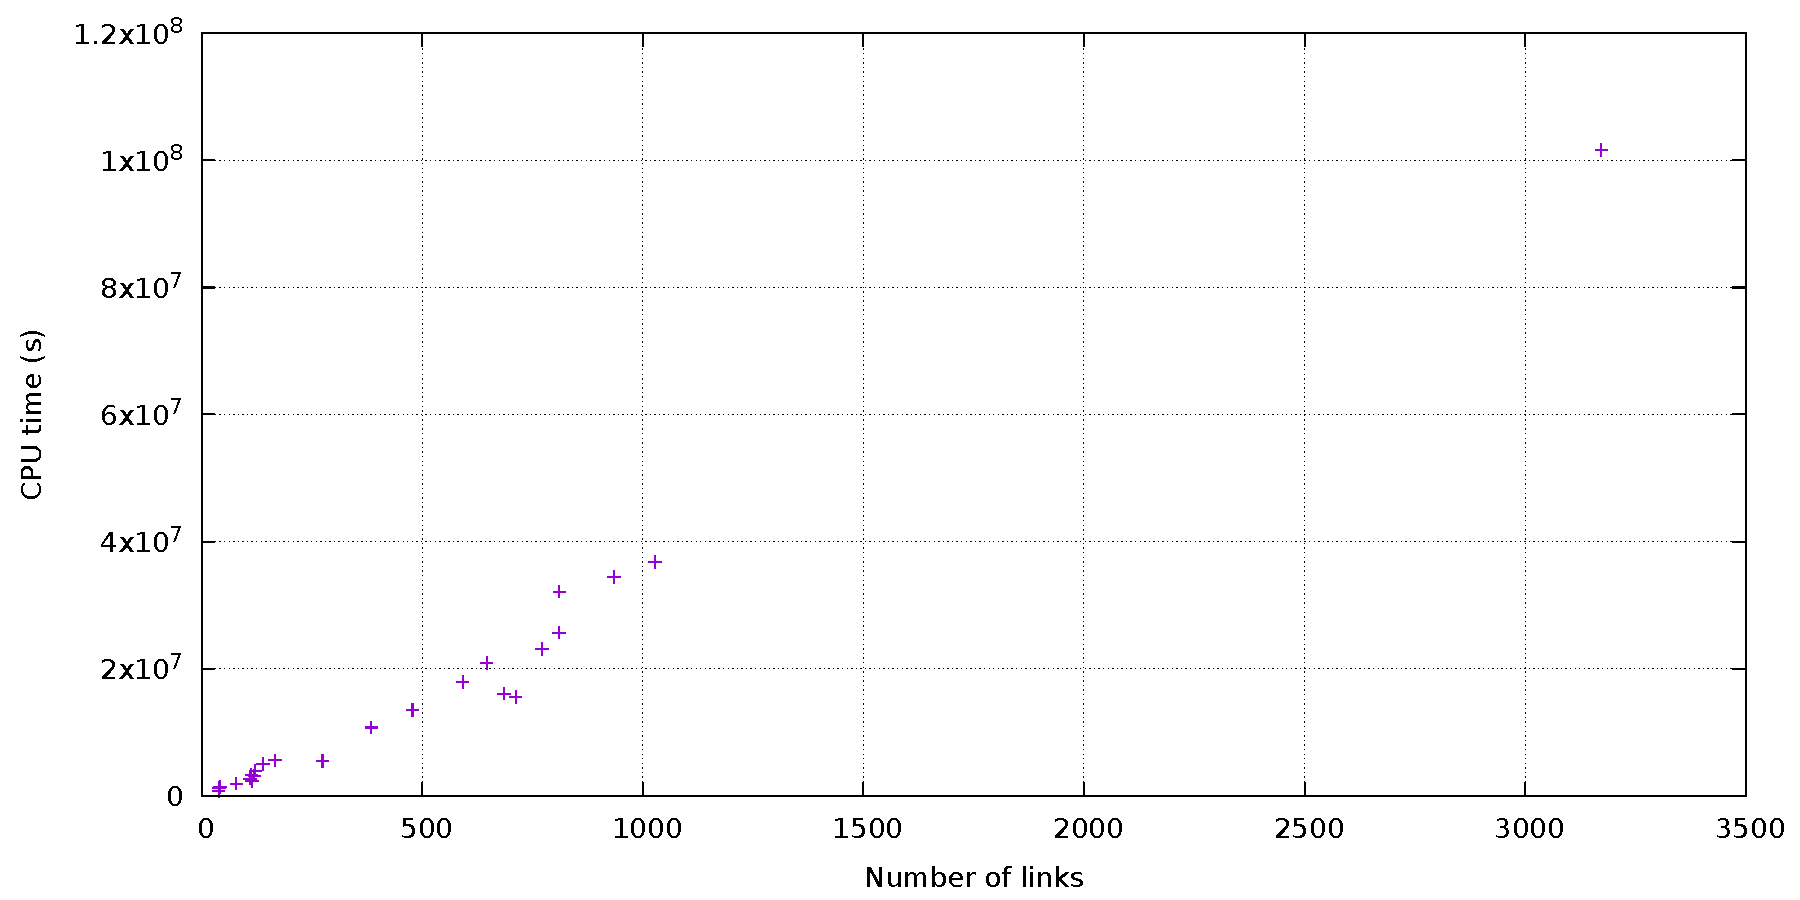
\includegraphics[width=.8\linewidth]{project/graph.pdf}
    \caption{CPU time in function of the number of links}
\end{figure}

There is an linear link between the number of links and the CPU time needed to compute the ranks. If we were to compute more data, the relation link/CPU time should follow this model.
\section{Conclusion}
In this project, the PageRank algorithm proved to be quite efficient. The results are satisfying despite a really long computation time.

There are several points that can be improved regarding the code:

As I used python, making use of the module \textbf{pandas} would have been faster to manipulate this amount of data. Python is also a slow language, reproducing the same code in fortran should be faster.
